\chapter{Results}

In this chapter, the results of the proposed algorithm are shown. The behaviour and performance is tested on an example scenario from the KITTI Vision Benchmark dataset. \cite{Geiger2013IJRR} Unfortunately no ground truth for any of the tracked objects is available, which is why the algorithm is evaluated visually only.

Since there are around $5-10$ tracked objects at any given time step, it is impossible to visualize the entire filter performance in this report in a satisfactory way. Instead, examples of characteristic and interesting filter behaviour are given and explained. Also a brief analysis of the estimation uncertainty of the extended target filter in comparison to a center point tracker is performed. This is done to emphasize the relative improvement in performance when using extended target models. Lastly, the computational complexity of the filter is analyzed and the benefit from using a neural network to split the measurement clusters into subsets is shown.

The best way to get an overview of the algorithm performance is to see it in real time. Therefore, a short ($22s$) video was created and uploaded to a hosting platform. The reader is encouraged to watch it before continuing in this chapter in order to get a better understanding of the subsequent explanations. \todo{video link}

\section{Scenario Description}
The scenario consists of 186 frames of lidar data in an urban area with pedestrians, cyclists and cars moving through the field of view. As outlined in the Thesis delimitations \todo{link}, the ego position is constant, the observed area is assumed to be a flat horizontal plane and a static map of the environment is available.

The area consists of a T-shaped intersection on which two cars and two bicycles will be observed during the scenario. There are also several sidewalks around the roads, and a crossing over one of them, on which pedestrians and groups of pedestrians can be seen throughout the entire example. An example frame of the scenario is shown in Figure \ref{fig:scenario_overview}.

\begin{figure}[H]
\centering
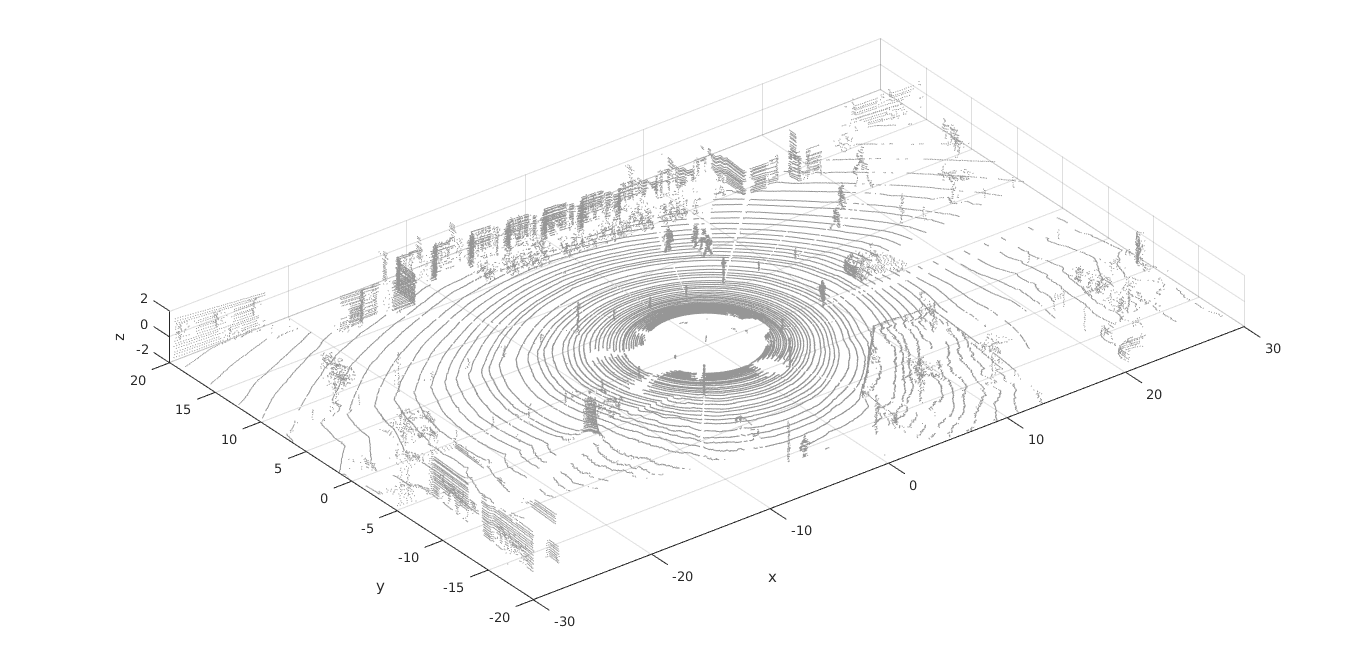
\includegraphics[width = \textwidth]{include/images/results_scenario_overview.png}
\caption{an overview of the test scenario area}
\label{fig:scenario_overview}
\end{figure}
\todo{actually draw the different parts as an overlay over the image to make the description clearer?}

\section{Algorithm Performance}
\subsection{Pre-Processing}
The several general pre-processing steps - ground removal, static map removal and clustering - aim to dismiss useless data and bundle the point data into objects. As pointed out in the description of these algorithms, all of them can be tuned between reducing the data as much as possible or keeping a high level of detail. 

For example, the clustering algorithm is parametrized by a minimum amount of points and a maximum distance between any two points in a cluster. The further an object is away from the lidar sensor, the fewer points it will consist of and the longer the distance between any two of these points will be. Setting a fixed threshold for the clustering parameters thus invariably leads to a decrease in the distance at which objects are tracked and identified by the implemented filter as opposed to the raw data.

An example of this can be seen in Figure \ref{fig:comp_dist_raw_cluster} which compares the raw point data of an example frame with the clusters derived from that data. In the raw data, the point that is furthest away from the sensor lies at a distance of about $100m$. In the clustered data this distance is reduced to about $50m$.

\begin{figure}[H]
\centering
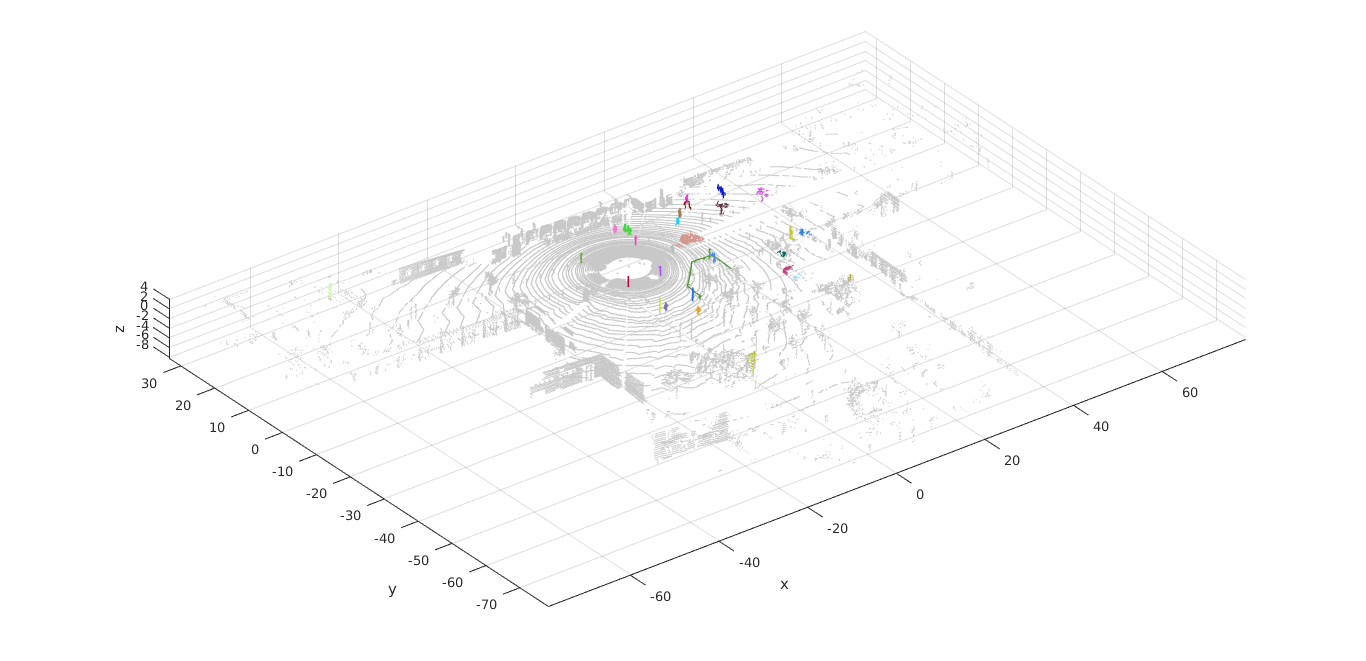
\includegraphics[width = \textwidth]{include/images/results_comp_dist_raw_cluster.png}
\caption{the difference in range of perception between raw data (gray) and clusters (colorful)}
\label{fig:comp_dist_raw_cluster}
\end{figure}

While this decrease in effective range is unfortunate, it is necessary to achieve a robust filter implementation. Both the neural network and the extended target tracking filters need objects with a certain minimum amount of points in order to derive distinct features (neural network) and extense measurements (tracker).
\todo{describe potential remedies? higher res sensor, dynamic clustering threshold, actually test with lower cutoff}

\subsection{Neural Network}
\todo{describe the nn hit rate}

\subsection{Tracking Filter}

The following examples are all taken from the test scenario described in the beginning of this chapter. Elliptical targets are displayed with a pink ellipse under the object cluster. Rectangular targets are shown as cuboid bounding boxes around the cluster. The classification of the different kinds of objects is visualized by a specific color value for all points in the cluster of that object. All clusters are drawn as an overlay over the original raw data to make orientiation in the scenario easier. The different colors can be seen in Table \ref{table:classification_legend}.

\begin{table}[H]
\centering
\begin{tabular}{ c | c c c c c c}
   Class & raw data & clutter & cars & cyclists & pedestrians & pedestrian groups\\
    \hline
    Color & 
    \tikz\draw[gray,fill=gray] (0,0) circle (.9ex); & 
    \tikz\draw[black,fill=black] (0,0) circle (.9ex); & 
    \tikz\draw[green,fill=green] (0,0) circle (.9ex); & 
    \tikz\draw[orange,fill=orange] (0,0) circle (.9ex); &
    \tikz\draw[cyan,fill=cyan] (0,0) circle (.9ex); &
    \tikz\draw[blue,fill=blue] (0,0) circle (.9ex);
\end{tabular}
\vspace{10pt}
\caption{legend showing the different colors used to visualize different classes of objects}
\label{table:classification_legend}
\end{table}

\subsubsection{Elliptical Filter}

The elliptical PHD filter manages to keep track of the multiple targets moving through the area of perception at any given time. Figure \ref{}

\todo{describe some interesting elliptical filter situations}

\subsubsection{Rectangular Filter}

During the scenario two non-stationary car are present. One of them (from now on referred to as Car 1) is present at the start of the scenario near the ego position, and drives in a more or less straight path before disappearing from sensor view. In total, Car 1 is present for 35 frames. The other one (Car 2) appears after approximately 20 frames, drives towards the ego car and later performs a $90^{\circ}$ turn, after which it drives away from the ego car and disappears from sensor view. In total, Car 2 is visible for 55 frames. 

Both cars are instantly detected by the PHD filter. Estimation of size, as well as position, velocity and heading all appear to be reasonable and follow the measurements in a steady manner. Estimation of size changes very little during the scenario, even though at some instances one only side of each car is seen. 

The rectangular PHD filter was tested with both an EKF and UKF when performing prediction and 

\todo{describe some interesting rectangular filter situations}

DUDE!

\section{Benefits of using Extended Targets}
Since no reference data is available evaluation of the algorithm performance 


\begin{figure}[ht]
    \begin{subfigure}{0.48\textwidth}
    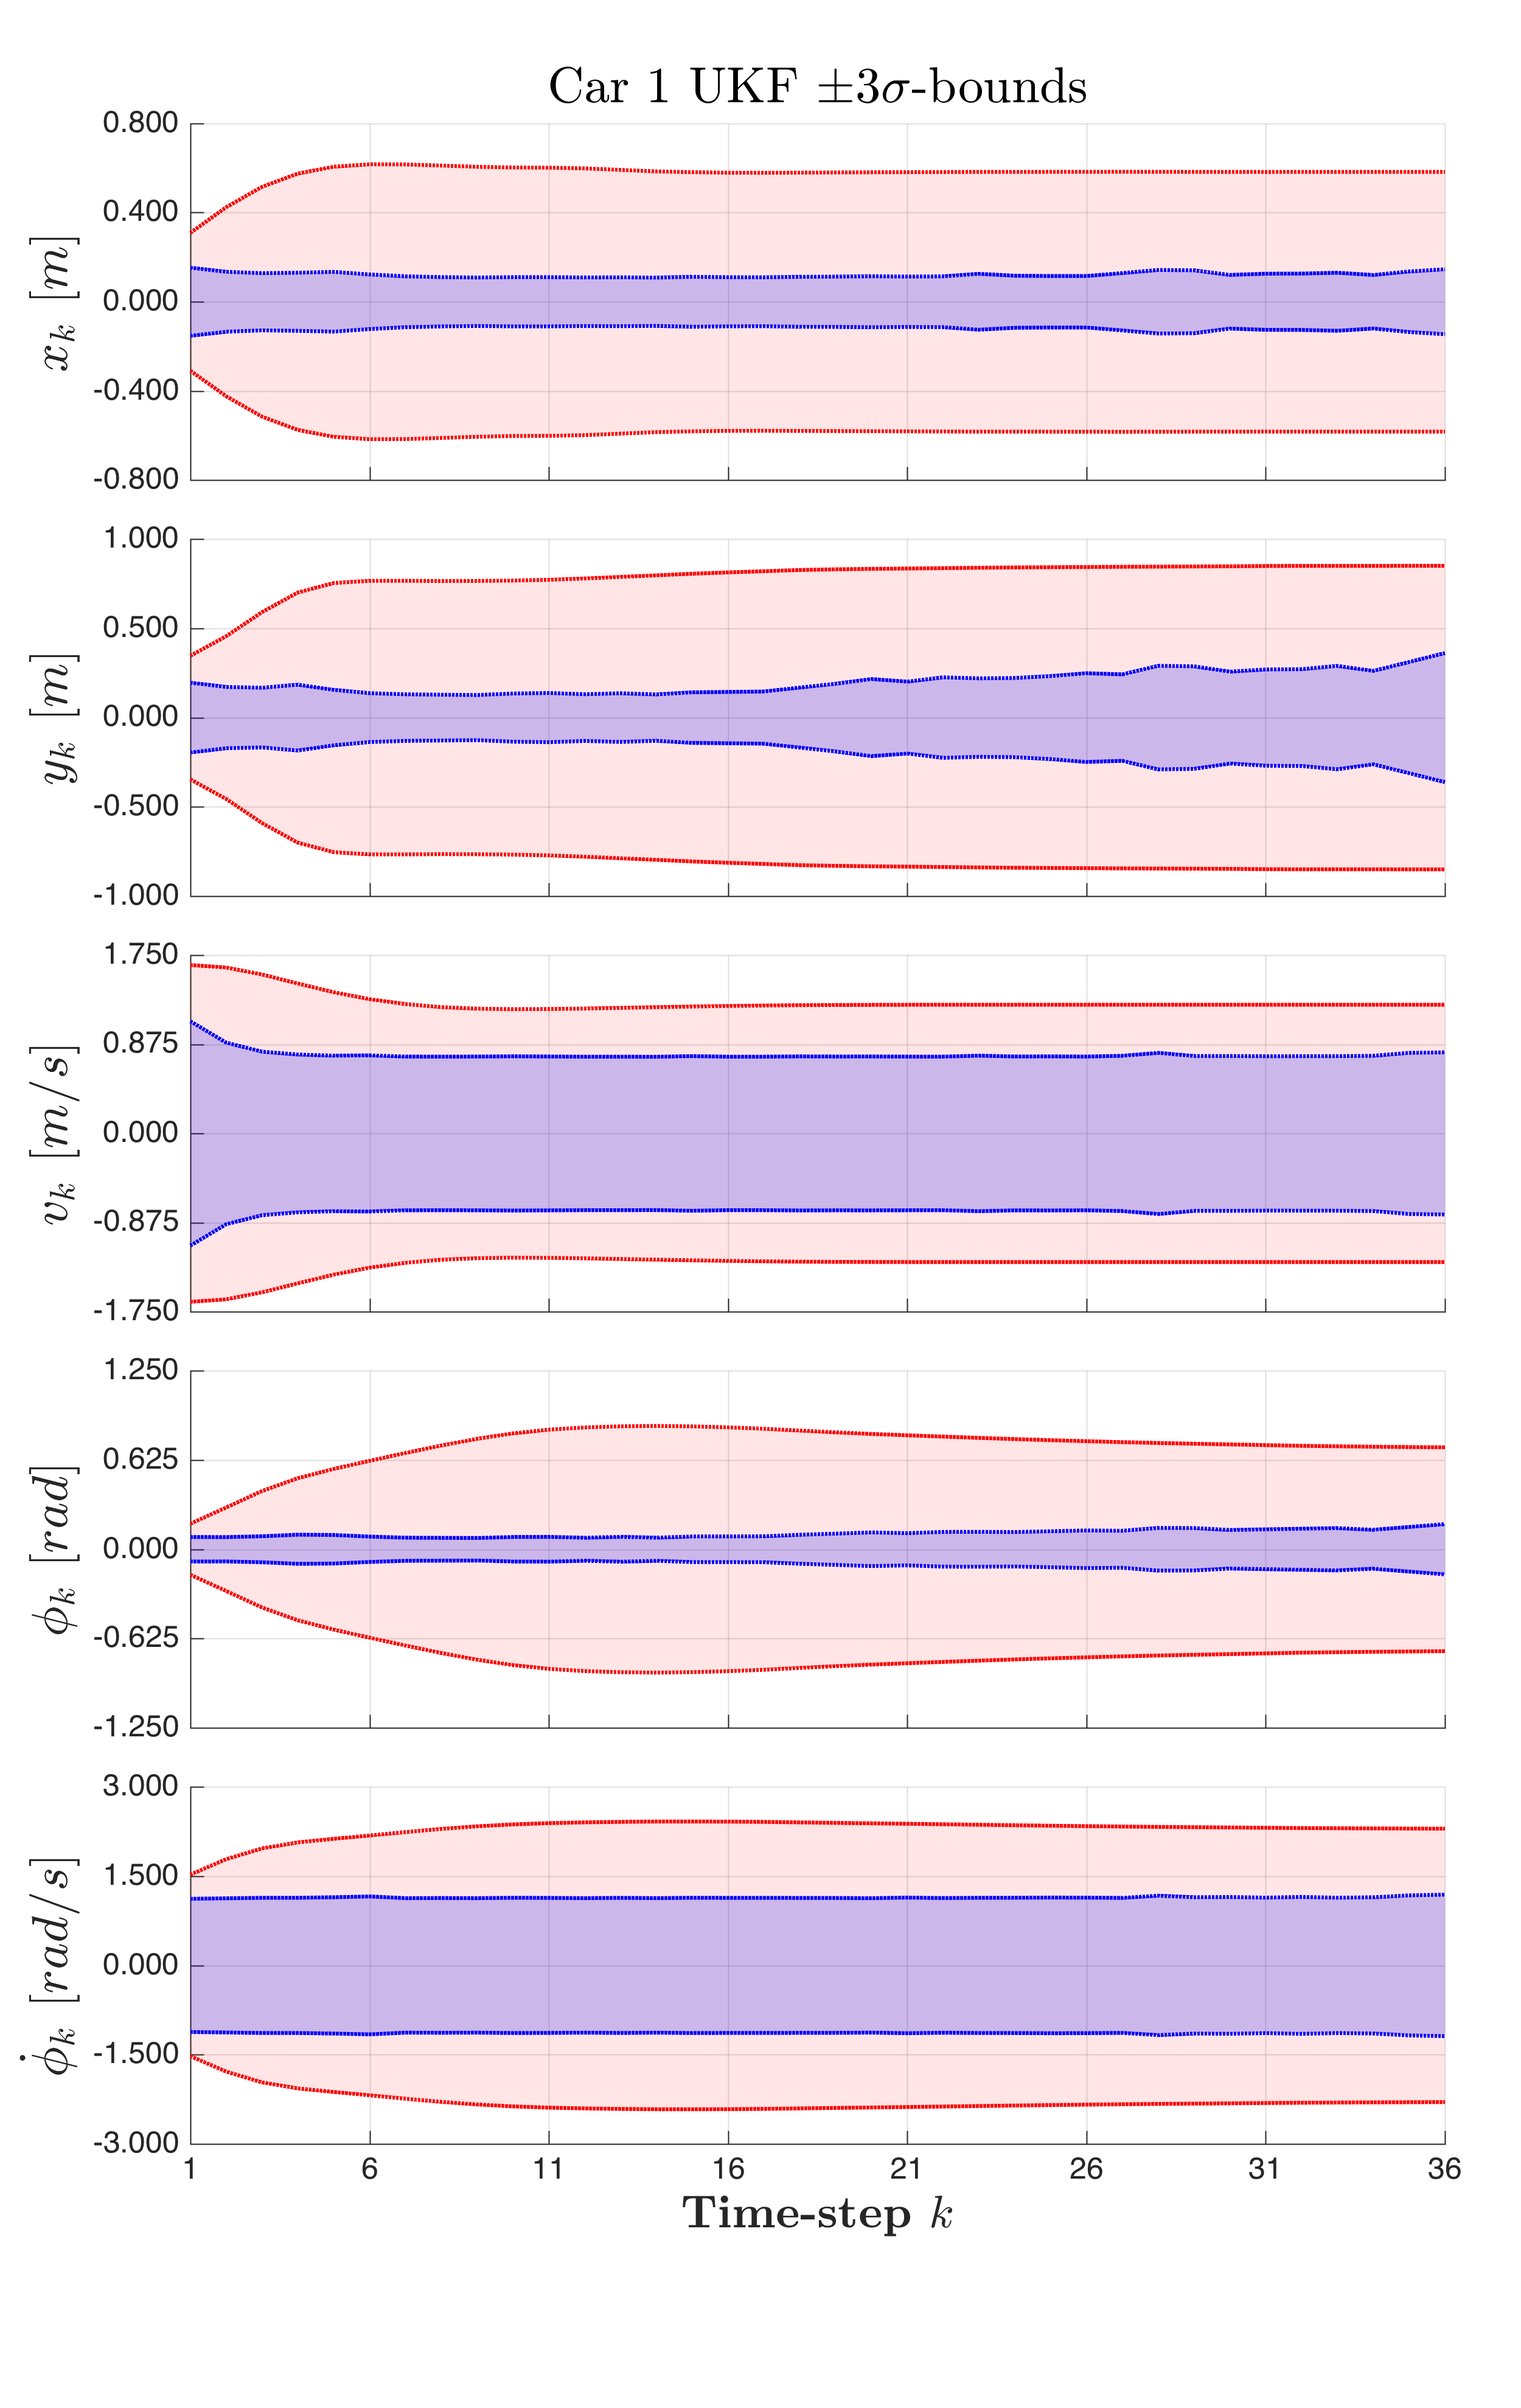
\includegraphics[width=0.9\linewidth]{include/images/car1.png} 
    \caption{Caption1}
    \label{fig:subim1}
    \end{subfigure}
    \begin{subfigure}{0.48\textwidth}
    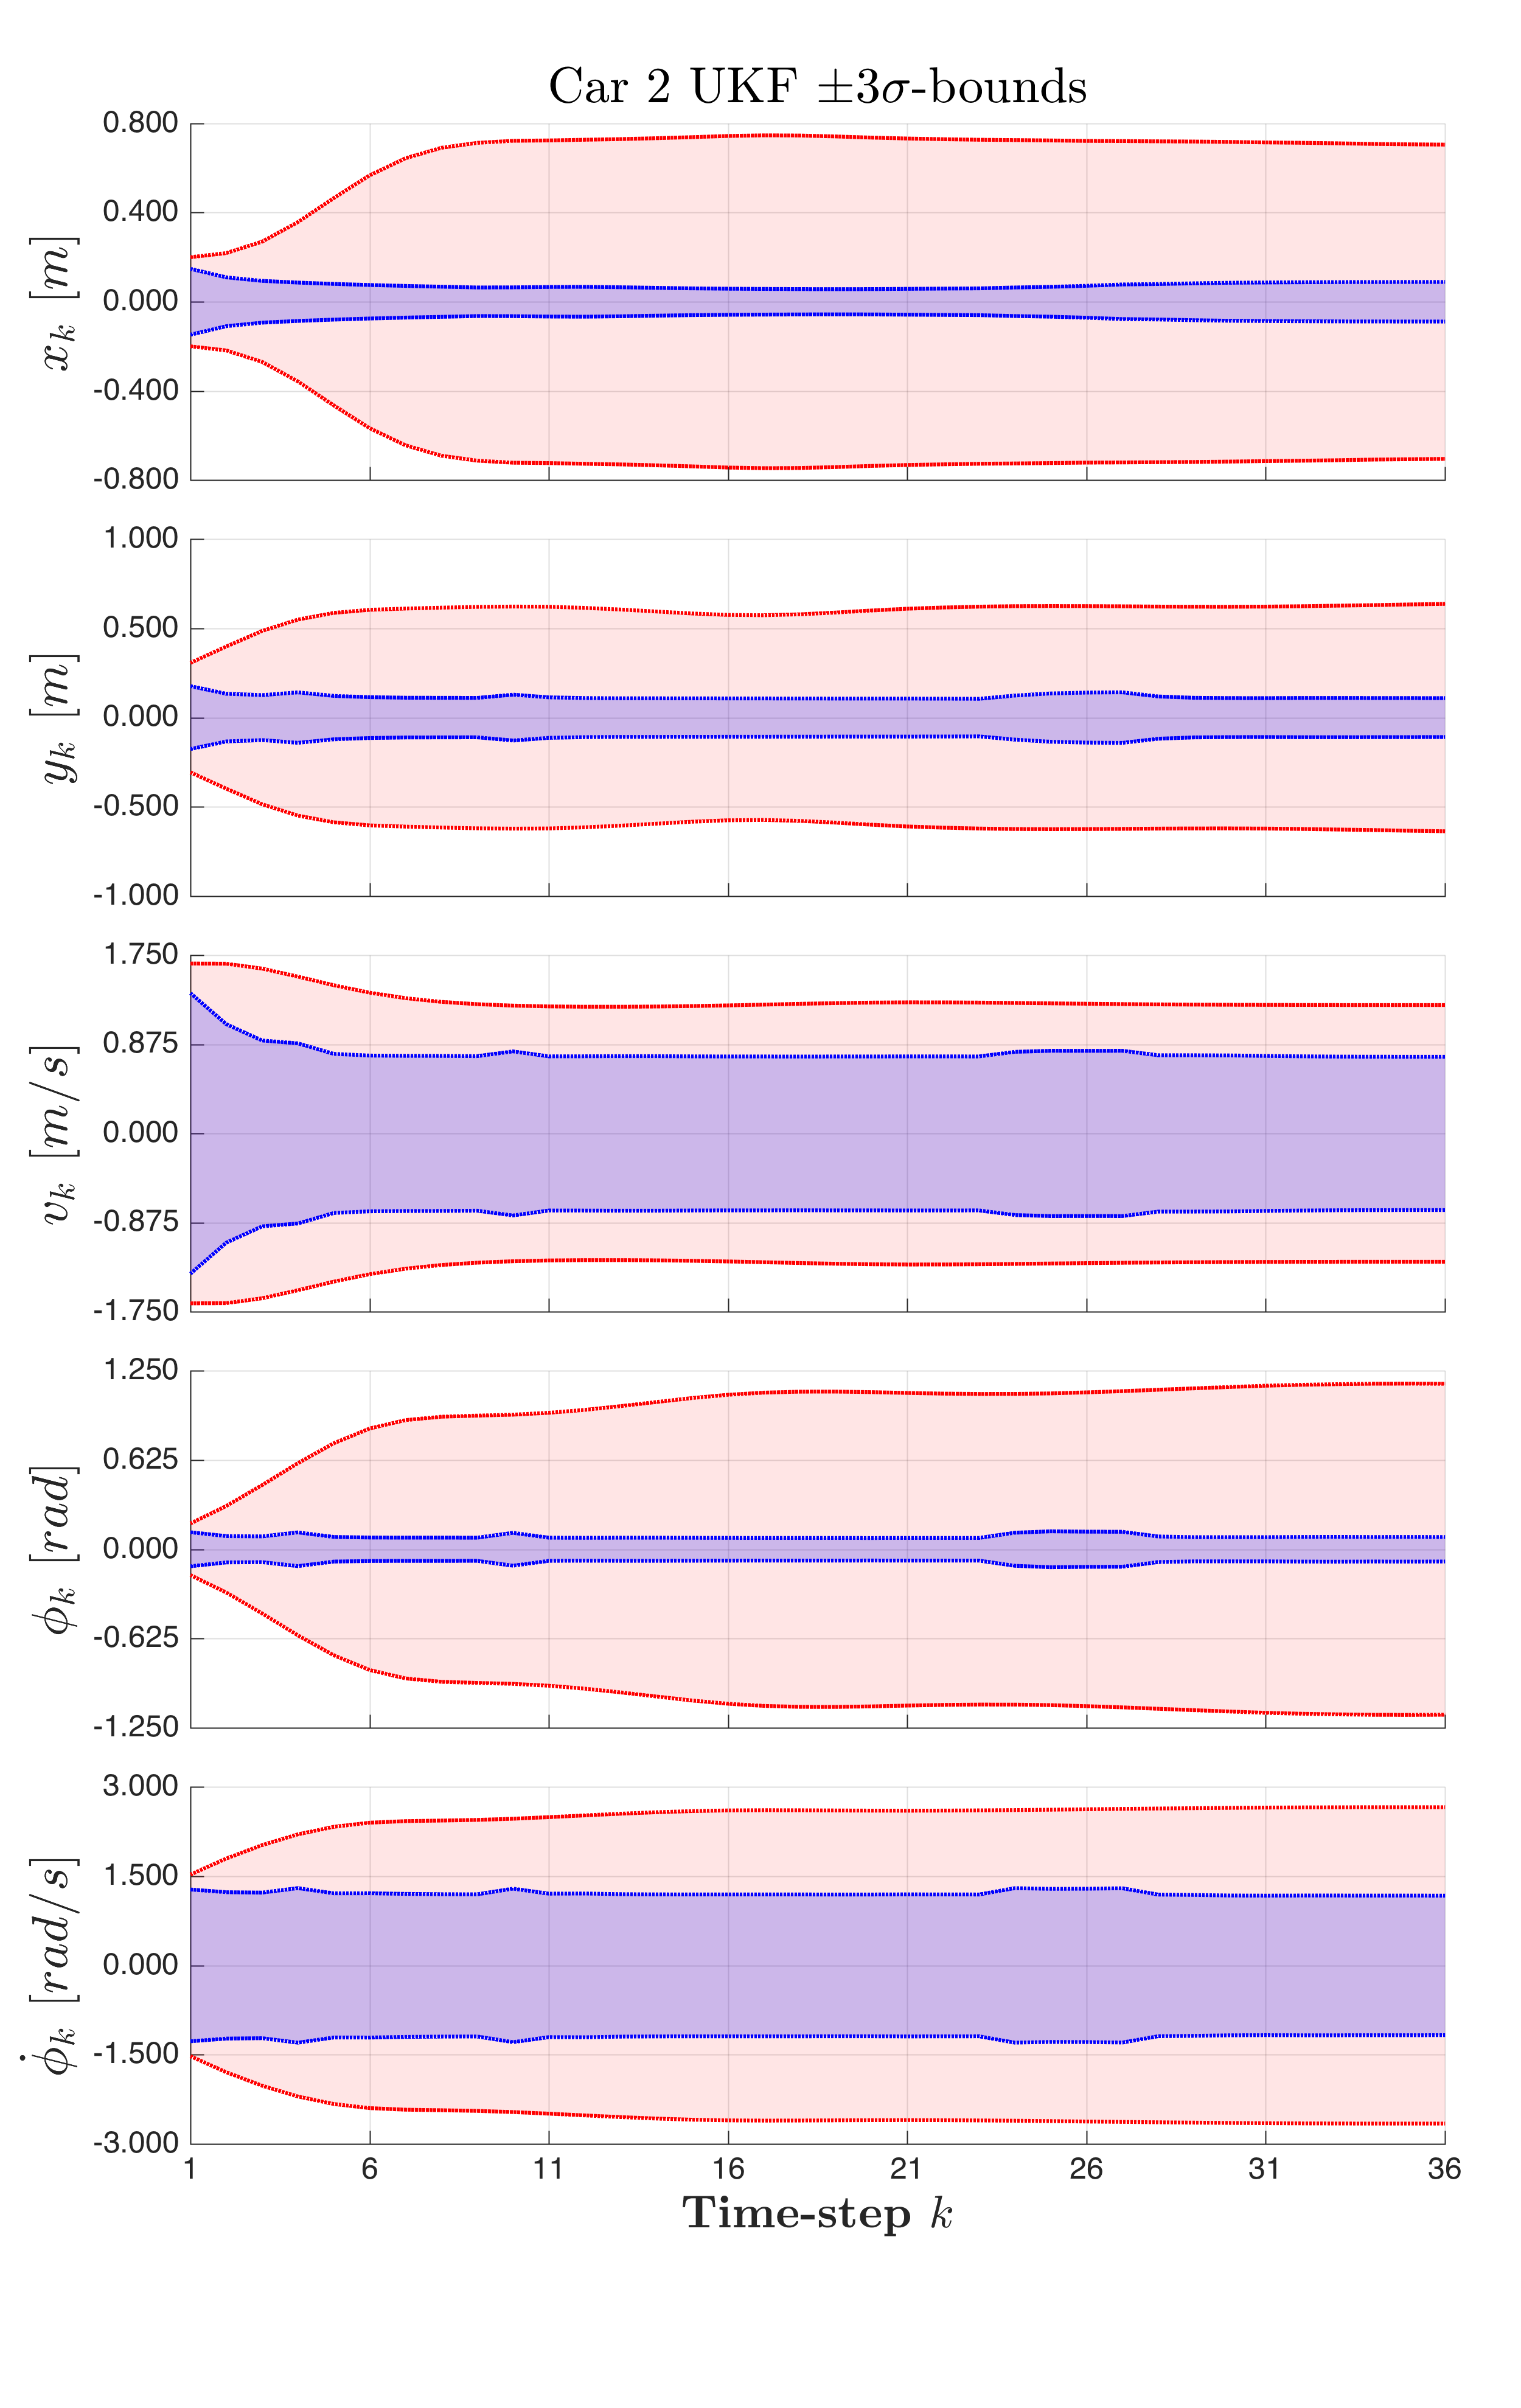
\includegraphics[width=0.9\linewidth]{include/images/car2.png}
    \caption{Caption 2}
    \label{fig:subim2}
    \end{subfigure}
     
    \caption{Caption for this figure with two images}
    \label{fig:image2}
\end{figure}

\begin{table}[ht]
    \centering
        \begin{tabular}{c|lr|lr}
            \multicolumn{1}{c}{} & \multicolumn{2}{c}{\underline{Car 1}} & \multicolumn{2}{c}{\underline{Car 2}} \\ [1mm]
            $RMS$ & ETT & PTT & ETT & PTT \\ [0.5mm]
            \hline
            $P_{xx}$                   & 0.060 &  1.330 & 0.044 &  2.716 \\ [0.25mm]
            $P_{yy}$                   & 0.179 &  2.511 & 0.087 &  2.522 \\ [0.25mm]
            $P_{vv}$                   & 2.418 &  6.758 & 3.809 & 10.349 \\ [0.25mm]
            $P_{\phi\phi}$             & 0.052 &  2.168 & 0.052 &  6.463 \\ [0.25mm]
            $P_{\dot{\phi}\dot{\phi}}$ & 5.198 & 20.998 & 8.763 & 39.379
        \end{tabular}
    \caption{Caption}
    \label{tab:my_label}
\end{table}



\section{Complexity Analysis}